\chapter{Experimental Framework}
\label{ch:Experiments}

In this chapter, I outline the setup for the experiments and describe the used datasets, models, evaluation methods and tools.

%%%%%%%%%%%%%%%%%%%%%%%%%%%%%%%%%%%%%%%%%%%%%%%%%%%%%%%%%%%%%%%%%%%%%%%%%%%%%%%%%%%%%%%%%%%%
\section{Languages}
\label{sec:Experiments:Languages}

% Source language: English 
% Target languages:
% - High resource: German (Germanic), French (Romance)
% - Low resource: Bulgarian (Slavic)

%%%%%%%%%%%%%%%%%%%%%%%%%%%%%%%%%%%%%%%%%%%%%%%%%
\subsection{Source Language} 
The source language used for translation is English, because translating from a notional gender language (English) into a grammatical gender language (e.g., German, French, Bulgarian) can produce biases by translating a non-gendered noun into the wrong gendered noun due to an unjustified assumption. Also, English is the most spoken language in the world, and many of the existing large datasets for training NMT models have English as either their source or target language.

%%%%%%%%%%%%%%%%%%%%%%%%%%%%%%%%%%%%%%%%%%%%%%%%%
\subsection{Target Language} 
The main target language for the base experiments of this study is German. This is primarily due to the writer's knowledge of the language, which leads to easier manual evaluation when necessary, as well as because the main occupational dataset, WinoMT \parencite{Stanovsky_2019}, also has gender evaluation for German.

% The experiments will be extended to other language families and lower-resource languages such as Bulgarian.

%%%%%%%%%%%%%%%%%%%%%%%%%%%%%%%%%%%%%%%%%%%%%%%%%%%%%%%%%%%%%%%%%%%%%%%%%%%%%%%%%%%%%%%%%%%%
\section{Datasets}
\label{sec:Experiments:Datasets}

% - test dataset for general MT model performance
% - test set (challenge set or natural corpora) for assessing gender bias

We use two types of datasets — challenge sets and natural corpora. Challenge sets are synthetically created sentences, designed to be used in a controlled experiment environment to evaluate a specific phenomenon. In contrast, natural corpora are comprised of naturally occurring sentences that are meant for training and testing phenomena in real-world scenarios.

%%%%%%%%%%%%%%%%%%%%%%%%%%%%%%%%%%%%%%%%%%%%%%%%%
\subsection{Challenge Test Set}
\label{sec:Experiments:Challenge_Set}

For detecting gender ambiguous words, we used the tagged challenge test set WinoMT, developed by \citet{Stanovsky_2019}. It consists of 3888 synthetic sentences presenting two human entities defined by their occupation and a subsequent pronoun that needs to be correctly resolved to match the gender of one of the entities. It also contains an equal balance between male and female gender nouns, as well as between stereotypical and non-stereotypical gender-role assignments (e.g., a female doctor versus a female nurse). We can see in Table \ref{tab:winomt} two sentences of the original dataset.

% - Downsides: synthetic samples - controlled experiment environment, but may introduce some artificial biases; only English as source language; too small set for training easy to overfit

\begin{table}
    \label{tab:winomt}
    \begin{tabularx}{\linewidth}{|X|l|l|l|}
        \hline
        \textbf{Source Sentence} & \textbf{Ambiguous word} & \textbf{Position} & \textbf{Gender} \\ \hline
        The \textbf{developer} argued with the designer because she did not like the design. & developer & 1 & female \\ \hline
        The developer argued with the \textbf{designer} because his idea cannot be implemented. & designer & 5 & male \\ \hline
    \end{tabularx}
    \caption{Example: WinoMT challenge set}
\end{table}

%%%%%%%%%%%%%%%%%%%%%%%%%%%%%%%%%%%%%%%%%%%%%%%%%
\subsection{Natural Corpora}
\label{sec:Experiments:Natural_Corpora}

In order to evaluate the approach in a natural setting, we used the natural multilingual corpus MuST-SHE \parencite{MuST-SHE}, designed to evaluate the performance of NMT systems in the translation of gender for English to Spanish/French/Italian. It comprises naturally occurring instances of spoken language retrieved from MuST-C \parencite{MuST-C}, which is built on TED Talks data. The samples in the dataset are balanced between masculine and feminine phenomena. They include sentences representing four different types of gender phenomena, which are classified based
on the type of information needed to disambiguate gender translation. We are specifically interested in the fourth category, which comprises sentences, for which no gender-disambiguating information can be retrieved from context, referred previously as \textit{unresolvable ambiguity}. It contains 34 sentences in total. In Table \ref{tab:mustshe} we can see two sentences of the category. 

\begin{table} 
    \label{tab:mustshe}
    \begin{tabularx}{\linewidth}{|X|l|l|}
        \hline
        \textbf{Source Sentence} & \textbf{Ambiguous Word} & \textbf{Gender} \\ \hline
        We have our cognitive biases, so that I can take a perfect history on a \textbf{patient} with chest pain. & patient & male \\ \hline
        And there was perpetual \textbf{victim} blaming when these victims came to report their crimes. & victim & female \\ \hline
    \end{tabularx}
    \caption{Example: MuST-SHE dataset}
\end{table}

%%%%%%%%%%%%%%%%%%%%%%%%%%%%%%%%%%%%%%%%%%%%%%%%%%%%%%%%%%%%%%%%%%%%%%%%%%%%%%%%%%%%%%%%%%%%
\section{NMT Models}
\label{sec:Experiments:Models}

We use the following pre-trained NMT models:

\subsection{English <-> German}
For translating into German, we rely on Fairseq's \footnote{https://github.com/facebookresearch/fairseq/blob/main/examples/wmt19/README.md} WMT’19 ensemble Transformer model, developed by Facebook \parencite{WMT19}. WMT is a MT dataset composed of a collection of various sources, including news commentaries and parliament proceedings. The corpus file has around 4M sentences, translated by professional translators.

% - French-English WMT’14 model, finetuned on MuST-C data to use for MuST-SHE evaluation

%%%%%%%%%%%%%%%%%%%%%%%%%%%%%%%%%%%%%%%%%%%%%%%%%%%%%%%%%%%%%%%%%%%%%%%%%%%%%%%%%%%%%%%%%%%%
\section{Evaluation Methods}
\label{sec:Experiments:Evaluation}

% TODO
% Evaluation procedures ought to cover both models’ general performance and gender-related issues. This is crucial to establish the capabilities and limits of mitigating strategies \cite{Savoldi_2021}.

% - Model performance metric: BLEU (translation quality)
% - Gender accuracy metric (gender bias)

%%%%%%%%%%%%%%%%%%%%%%%%%%%%%%%%%%%%%%%%%%%%%%%%%%%%%%%%%%%%%%%%%%%%%%%%%%%%%%%%%%%%%%%%%%%%
\section{Technical Details}
\label{sec:Experiments:Technical}

%%%%%%%%%%%%%%%%%%%%%%%%%%%%%%%%%%%%%%%%%%%%%%%%%
\subsection{Tools}
\label{sec:Experiments:Tools}

In this section, we mention the most used tools during the development of the experiments. The programming code for the experiments is written in Python, and we use PyTorch's library for deep learning.

\paragraph{Pre-processing Tools:}
\begin{itemize}
    \item \textbf{Sacremoses \footnote{https://github.com/alvations/sacremoses}:} A pre-porcessing tool for the tokenization and de-tokenization of text.
    \item \textbf{Subword NMT \footnote{https://github.com/rsennrich/subword-nmt}:} A pre-processing tool for segmenting text into subword units. % used for the French models
    \item \textbf{Fast BPE \footnote{https://github.com/glample/fastBPE}:} A pre-processing tool for segmenting text into subword units. % used for the German models
    \item \textbf{Spacy \footnote{https://spacy.io/}:} An open-source library for Natural Language Processing. We use it for the detection of stop words, lemmatization and prediction of gender.
\end{itemize}

\paragraph{Word Alignment Tools:}
\begin{itemize}
    \item \textbf{Fast align \footnote{https://github.com/clab/fast\_align}:} A simple and fast unsupervised word aligner developed by \citet{fast-align}. This tool is used to align the translated sentences with the source sentences.
    \item \textbf{Awesome align \footnote{https://github.com/neulab/awesome-align}:} A tool, developed by \citet{awesome-align}, that can extract word alignments from multilingual BERT (mBERT) and allows you to fine-tune mBERT on parallel corpora for better alignment quality. We use the default mBERT model provided in the package to align the source sentences with the translated sentences.
    \item \textbf{Tercom alignment \footnote{https://github.com/jhclark/tercom}:} A tool for aligning between different translations of the source sentence. We use it to align the source sentences with the corresponding backtranslations.
\end{itemize}

%%%%%%%%%%%%%%%%%%%%%%%%%%%%%%%%%%%%%%%%%%%%%%%%%
\subsection{Hardware Resources}
\label{sec:Experiments:Hardware}

% TODO
% - GPU: GeForce GTX 1080 Ti
% - Batch size
% - Training time

%%%%%%%%%%%%%%%%%%%%%%%%%%%%%%%%%%%%%%%%%%%%%%%%%%%%%%%%%%%%%%%%%%%%%%%%%%%%%%%%%%%%%%%%%%%%
\section{Experimental Procedure}
\label{sec:Experiments:Procedure}

We follow three main steps in doing the experiments. First, we preprocess the data, then we translate it, and lastly we evaluate the translations based on different factors.

%%%%%%%%%%%%%%%%%%%%%%%%%%%%%%%%%%%%%%%%%%%%%%%%%
\subsection{Data Pre-processing}

As we can see in Subsection \ref{sec:Experiments:Challenge_Set}, the sentences in WinoMT usually consist of two gender ambiguous occupations and a context, containing disambiguation information about one of the occupations. We take the following steps to preprocess the sentences:

\begin{enumerate}
  \item \textbf{Sentence Extraction:}  
  In order to obtain fully ambiguous sentences, we remove the context information from the sentences and obtain a subset of 335 sentences from the type: "The developer argued with the designer.".
  To remove additional detection overhead, we want to have a single ambiguous word per sentence. For this purpose, we replace the second ambiguous word with a non-ambiguous proper noun, e.g. "John". 
  \item \textbf{Disambiguation:} 
  As next, we generate a new set of sentences, replacing the ambiguous word with a disambiguated version. We disambiguate the ambiguous word with different techniques:
  \begin{itemize}
      \item \textbf{Gender Forcing:} We use the gender-defining adjectives \textit{male} and \textit{female} in front of the gender-ambiguous word. This technique is meant to force the translator to make the right decision regarding gender.
      \item \textbf{Common Words Disambiguating:} We replace the ambiguous word with the following common gender non-ambiguous words: \textit{man, woman, girl, guy, boy}. This method serves as a baseline for comparison against the disambiguated occupations.
  \end{itemize}
\end{enumerate}

Table \ref{tab:preprocessing} shows the generated subsets obtained by disambiguating the base ambiguous sentence "The developer argued with John.".

\begin{table}
    \label{tab:preprocessing}
    \begin{tabularx}{\linewidth}{|l|X|}
        \hline
        \textbf{Disambiguation Method} & \textbf{Source Sentence} \\ \hline
        Gender Forcing & The \textbf{male developer} argued with John. \newline
        The \textbf{female developer} argued with John. \\ \hline
        Common Words & The \textbf{man} argued with John. \newline
        The \textbf{woman} argued with John. \newline
        The \textbf{girl} argued with John. \newline
        The \textbf{guy} argued with John. \newline
        The \textbf{boy} argued with John. \\ \hline
    \end{tabularx}
    \caption{Example: Disambiguation subsets for the baseline sentence "The developer argued with John."}
\end{table}

%%%%%%%%%%%%%%%%%%%%%%%%%%%%%%%%%%%%%%%%%%%%%%%%%
\subsection{Translation}

The next step in conducting the experiments is translating the subsets of sentences. This is executed in two steps:

\begin{enumerate}
    \item \textbf{Translation Source -> Target:} 
    First, the subsets are translated in the target language.
    \item \textbf{Backtranslation Target -> Source:}
    The second step involves translating the translations back into the source language.
\end{enumerate}


% TODO: Decoding/search algorithm/strategy, nbest size
% We use two different decoding algorithms to compare the results: Beam search and Sampling. 
% In each step we generate nbest lists of different sizes: 10 and 100.

% ! \citet{roberts2020decoding} prove that beam search unlike sampling is skewed toward the generation of more frequent (masculine) pronouns, as it leads models to an extreme operating point that exhibits zero variability.

%%%%%%%%%%%%%%%%%%%%%%%%%%%%%%%%%%%%%%%%%%%%%%%%%
\subsection{Evaluation}

The last step in the experiments involves evaluating the translations and backtranslations to detect patterns using different statistical methods.

%%%%%%%%%%%%%%%%%%%%%%%%%
\subsubsection{Word alignment}
\label{sec:Experiments:Alignment}

First, in order to assign the words in the source sentence to their counterparts in the translations, we use two different alignment methods:

\begin{enumerate}
    \item Source-to-translation (\textit{fast\_align}, \textit{awesome-align}): This alignment method aligns from the source language to the target language.
    \item Translation-to-translation (\textit{Tercom}): This alignment method aligns between two translations.
\end{enumerate}

We use the first method to map each word in the source sentence to its translations and backtranslations in the target nbest lists. We do this in a two-step way, depicted in Fig. \ref{fig:alignment}. First, we align between the source sentence and the sentences in the nbest translations and extract the translations for each word. Then, we align between the translations and the backtranslations and extract the corresponding backtranslations resulting from the aligned translations of each word. 

We use the results from the second method as a baseline for comparison with the first method and to detect possible errors, which may occur in the information transfer between the two steps in the first method.

\begin{figure}
  \centering
  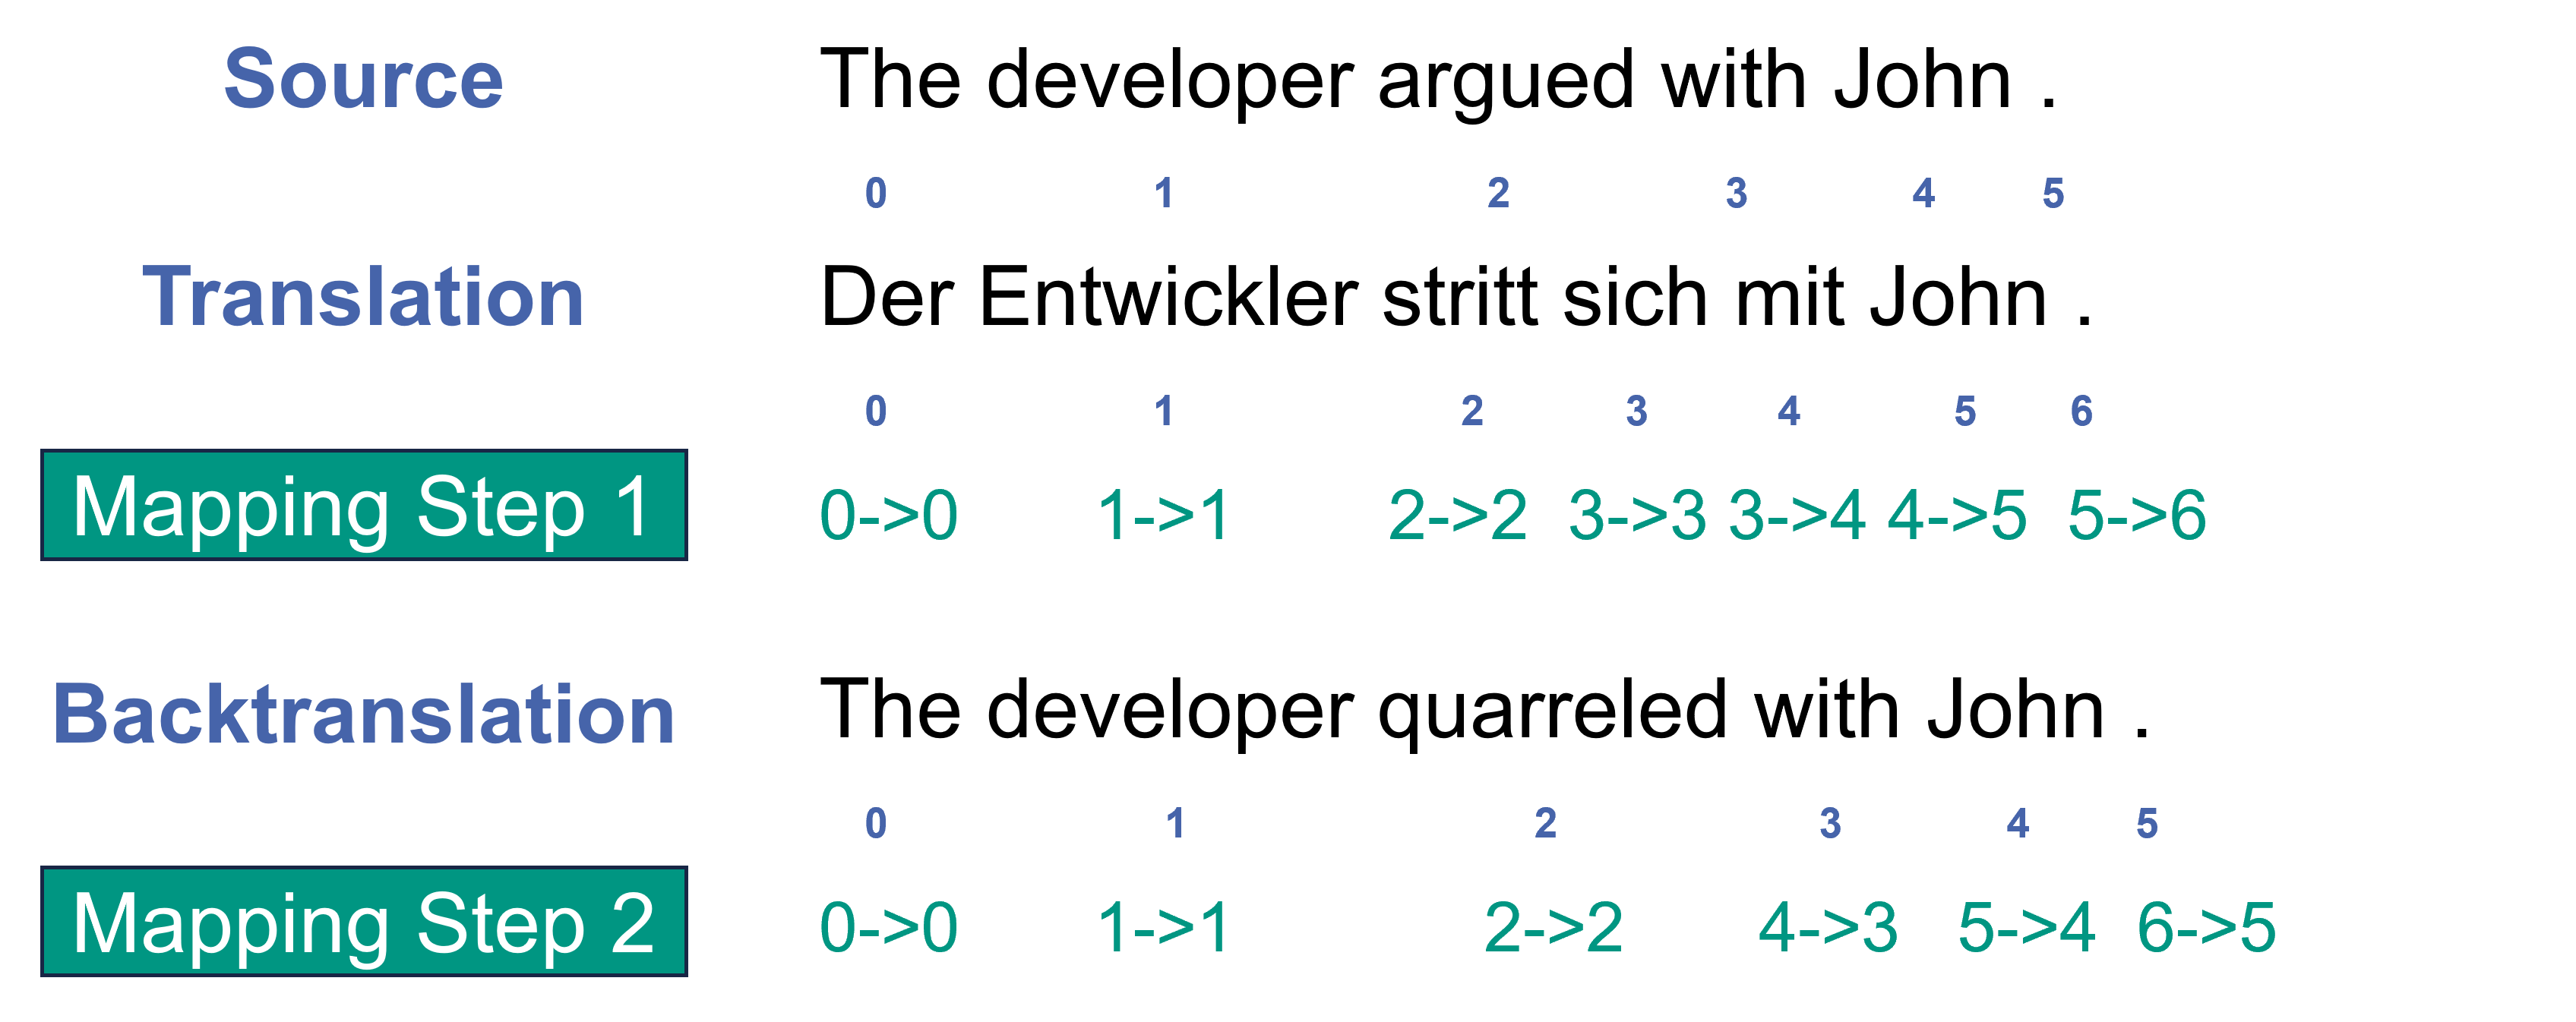
\includegraphics[scale=0.5]{figures/alignment.png}
  \caption{Example Illustration: 2-step mapping from source to translation and backtranslation}
  \label{fig:alignment}
\end{figure}

%%%%%%%%%%%%%%%%%%%%%%%%%
\subsubsection{Statistics}
\label{sec:Experiments:Statistics}



% Statistics on test set: !!! define formally, maybe as a formula
% - Gender produced in translation: for each source sentence how many of them produce both genders, male gender and female gender in translations
% - Reoccurrence: how often ambiguous word reoccurs in backtranslation; for each source sentence how many of the sentences/ambiguous words reoccur in backtranslations
% - Uniqueness: 
% -- sentence level: out of the 100 backtranslated sentences to each source sentence how many are unique
% -- word level: how many unique words in translation vs. backtranslation
% - Word occurrence: Check number of unique words for each word in sentence: non-ambiguous words such as stop words like “the” should have less unique translations 
% - Word alignment: out of 10 translations/backtranslations to each source sentence how many unique words to the ambiguous words are produced





